\documentclass[paper=a4,fontsize=10pt,jafontscale=0.92]{jlreq}

%% --- パッケージ ---
\usepackage{amsmath,amssymb,amsthm}
\usepackage{mathtools}
\usepackage{ebproof}
\usepackage{booktabs}
\usepackage{xcolor}
\usepackage[most]{tcolorbox}
\usepackage{tikz}
\usetikzlibrary{arrows.meta,positioning,fit,backgrounds,calc,decorations.pathreplacing}
\usepackage{hyperref}
\hypersetup{colorlinks=true,linkcolor=blue!60!black,urlcolor=blue!60!black}

%% --- 定理環境 ---
\theoremstyle{plain}
\newtheorem{theorem}{定理}
\newtheorem{lemma}[theorem]{補題}
\newtheorem{corollary}[theorem]{系}
\theoremstyle{definition}
\newtheorem{definition}[theorem]{定義}
\theoremstyle{remark}
\newtheorem*{remark}{注意}

%% --- 検証ブロック ---
\tcbuselibrary{skins,breakable}
\newtcolorbox{verifybox}{
  breakable,
  enhanced,
  colback=gray!7,
  colframe=gray!45,
  boxrule=0.5pt,
  arc=2pt,
  left=8pt, right=8pt, top=5pt, bottom=5pt,
  before skip=6pt, after skip=6pt,
  fontupper=\small,
}

%% --- tikz スタイル定義 ---
% occurrence nodes
\tikzset{
  occ/.style={circle,draw,inner sep=2.2pt,font=\scriptsize\strut},
  vis/.style={occ,fill=blue!15,draw=blue!55,thick},
  inv/.style={occ,fill=orange!18,draw=orange!65},
  % trace edges
  traceedge/.style={thick,gray!55,-{Stealth[length=4pt,width=3.5pt]}},
  traceedgebi/.style={thick,gray!55,{Stealth[length=4pt,width=3.5pt]}-{Stealth[length=4pt,width=3.5pt]}},
  % piece highlights
  pieceA/.style={draw=teal!55,dashed,thick,rounded corners=4pt},
  pieceB/.style={draw=red!55,dashed,thick,rounded corners=4pt},
  pieceC/.style={draw=violet!55,dashed,thick,rounded corners=4pt},
  % derivation tree nodes
  cat/.style={font=\small},
  % band contraction
  bandbox/.style={draw=red!50,fill=red!6,rounded corners=2pt},
  % branch zone diagram
  zonebox/.style={fill=yellow!18,draw=yellow!60,rounded corners=2pt},
  vismark/.style={fill=blue!20,draw=blue!50,rounded corners=1pt},
  invmark/.style={fill=orange!20,draw=orange!50,rounded corners=1pt},
}

%% --- マクロ ---
\newcommand{\R}{\mathcal{R}}
\newcommand{\Sig}{\Sigma}
\newcommand{\At}{\operatorname{At}}
\newcommand{\Occ}{\operatorname{Occ}}
\newcommand{\Chart}{\mathsf{Chart}}
\newcommand{\st}{\operatorname{st}}
\newcommand{\bs}{\backslash}
\newcommand{\Dmin}{D_{\min}}

%% --- 本文 ---
\begin{document}

\title{八規則 CCG の導出可能性は判定可能である\\
  \large ——unrestricted type raising を含む体系の自己完結な決定可能性証明}
\author{}
\date{}
\maketitle

\begin{abstract}
本稿は，unrestricted type raising を含む八規則 Combinatory Categorial Grammar (CCG) において，
導出可能性が判定可能であることを自己完結に証明する．
論証中の主要な構成（valid な導出，trace graph，invisible piece，band contraction，深さ上界の数え上げ）
はすべて実際に計算機で検算した具体例で裏付けてあり，
tikz による図と ebproof による導出木で可視化してある．
\end{abstract}

\tableofcontents

%% ============================================================
\section*{主定理}
\addcontentsline{toc}{section}{主定理}
%% ============================================================

入力範疇列 $\Gamma = x_1, \ldots, x_n$ と目標範疇 $y$ が与えられたとき，
\[
  x_1, \ldots, x_n \Rightarrow_{\R}^{*} y
\]
が成り立つかどうかは判定可能である．ただし規則集合は
\[
  \R = \{{\mathbin{<}},\,{\mathbin{>}},\,T{\mathbin{<}},\,T{\mathbin{>}},\,B{\mathbin{<}},\,B{\mathbin{>}},\,Bx{\mathbin{<}},\,Bx{\mathbin{>}}\}
\]
である．範疇は $A ::= p \mid A/B \mid A\bs B$ で生成される．

\medskip
\noindent\textbf{証明の大構造．}
証明は四段階からなる．
\begin{enumerate}
  \item \textbf{原子消去（補題~\ref{lem:atom}）}：入力と目標に現れない原子は準同型で潰せる．原子集合を有限集合 $\Sig$ に固定できる．
  \item \textbf{Band-contraction（補題~\ref{lem:band-correct}--\ref{lem:band-contract}）}：「外から見えない繰り返し」は縮約でき，constructor occurrence 総数 $\mu$ を真に減らせる．ゆえに $\mu$-最小成功導出には repeatable pair が存在しない（系~\ref{cor:minimal}）．
  \item \textbf{深さ上界（\S\ref{sec:depth}）}：$\mu$-最小成功導出の中間範疇の深さは，入力と目標から計算できる有限量 $H(\Gamma, y)$ で有界．
  \item \textbf{有限 chart parsing（\S\ref{sec:chart}）}：深さ有界より候補範疇集合 $K_{\Gamma,y}$ が有限．標準的な chart algorithm が停止し，健全かつ完全．
\end{enumerate}
技術的核心はステップ 2 であり，その正当性はステップ 3 の数え上げで使われる．

%% ============================================================
\part{規則と導出図}
%% ============================================================

\section{八規則}

下表に八規則を ebproof の導出木形式で示す．横線の右に規則名を添える．

\begin{center}
\setlength{\tabcolsep}{18pt}
\renewcommand{\arraystretch}{1.6}
\begin{tabular}{@{}cc@{}}
% row 1
\begin{prooftree}
  \hypo{C/B} \hypo{B}
  \infer2[$(>)$]{C}
\end{prooftree}
&
\begin{prooftree}
  \hypo{A} \hypo{A\bs C}
  \infer2[$(<)$]{C}
\end{prooftree}
\\
% row 2
\begin{prooftree}
  \hypo{A}
  \infer1[$(T{>})$]{C/(A\bs C)}
\end{prooftree}
&
\begin{prooftree}
  \hypo{A}
  \infer1[$(T{<})$]{(C/A)\bs C}
\end{prooftree}
\\
% row 3
\begin{prooftree}
  \hypo{C/B} \hypo{B/A}
  \infer2[$(B{>})$]{C/A}
\end{prooftree}
&
\begin{prooftree}
  \hypo{A\bs B} \hypo{B\bs C}
  \infer2[$(B{<})$]{A\bs C}
\end{prooftree}
\\
% row 4
\begin{prooftree}
  \hypo{C/B} \hypo{A\bs B}
  \infer2[$(Bx{>})$]{A\bs C}
\end{prooftree}
&
\begin{prooftree}
  \hypo{B/A} \hypo{B\bs C}
  \infer2[$(Bx{<})$]{C/A}
\end{prooftree}
\end{tabular}
\end{center}

型上げ規則 $T{>},\,T{<}$ における $C$ は\textbf{任意の範疇}である．
これが unrestricted type raising であり，中間範疇が無限に深くなりうる原因である．

\section{導出図}

\textbf{導出図} $D$ とは，有限木であって，各節点に範疇がラベルされ，
各内部節点が八規則のいずれかのインスタンスであるものをいう．
葉は左から順に $x_1, \ldots, x_n$，根は目標範疇 $y$ である．

二項規則は隣接する二区間を結合する．入力長 $n$ の導出では二項規則の使用回数は常に $n-1$ である．型上げは unary rule であり葉数を変えない．

\begin{verifybox}
\textbf{【例1：具体的な成功導出】}
入力 $a,\;(a\bs s)/b,\;b$ から目標 $s$ への導出（$T{>}$ + $B{>}$ + $>$）：

\medskip
\begin{center}
\begin{prooftree}
  \hypo{a}
  \infer1[$(T{>},\;C{=}s)$]{s/(a\bs s)}
  \hypo{(a\bs s)/b}
  \infer2[$(B{>})$]{s/b}
  \hypo{b}
  \infer2[$(>)$]{s}
\end{prooftree}
\end{center}
\end{verifybox}

\begin{verifybox}
\textbf{【例1$'$：言語学的な例 ``John loves Mary'' と spurious ambiguity】}
語彙を $\text{John}=np$，$\text{loves}=(np\bs s)/np$，$\text{Mary}=np$，目標 $s$ とする．
同じ入力列に対して，型上げを使わない導出（A）と主語型上げ＋合成を使う導出（B）の
\textbf{二通り}が存在し，いずれも目標 $s$ に到達する（CCG に特有の spurious ambiguity）．
両者とも計算機で valid 確認済み．

\medskip
\begin{center}
\begin{tabular}{cc}
\textbf{導出A（型上げなし）} & \textbf{導出B（主語型上げ＋合成）} \\[4pt]
\begin{prooftree}
  \hypo{np}
  \hypo{(np\bs s)/np}
  \hypo{np}
  \infer2[$(>)$]{np\bs s}
  \infer2[$(<)$]{s}
\end{prooftree}
&
\begin{prooftree}
  \hypo{np}
  \infer1[$(T{>})$]{s/(np\bs s)}
  \hypo{(np\bs s)/np}
  \infer2[$(B{>})$]{s/np}
  \hypo{np}
  \infer2[$(>)$]{s}
\end{prooftree}
\end{tabular}
\end{center}

\smallskip
導出 B では型上げが中間範疇 $s/(np\bs s)$ を生む．この種の「同一目標への複数経路」が
unrestricted type raising の下では無限に増えうるため，深さの有界化が必要になる．
\end{verifybox}

%% ============================================================
\part{原子の有限化}
%% ============================================================

\section{原子消去補題}
\label{sec:atom}

\begin{definition}
入力と目標に現れる原子の集合を
$\Sig = \At(x_1) \cup \cdots \cup \At(x_n) \cup \At(y)$
と定める．
\end{definition}

\begin{lemma}[原子消去補題]
\label{lem:atom}
$x_1, \ldots, x_n \Rightarrow_{\R}^{*} y$ が成り立つなら，途中に現れる原子がすべて $\Sig$ に属する導出が存在する．
\end{lemma}

\begin{proof}
$\Sig$ から原子 $p_\ast$ を一つ選び，原子上の写像 $h$ を
\[
  h(p) = \begin{cases} p & p \in \Sig,\\ p_\ast & p \notin \Sig \end{cases}
\]
と定め，$h(A/B) = h(A)/h(B)$，$h(A\bs B) = h(A)\bs h(B)$ と準同型拡張する．
各規則はスキーム規則なので，規則適用が成り立つなら $h$ をかけたものも同じ規則適用である．たとえば $B{>}$ では
\[
  C/B,\;B/A \Rightarrow C/A
  \;\xrightarrow{\;h\;}\;
  h(C)/h(B),\;h(B)/h(A) \Rightarrow h(C)/h(A)
\]
で再び $B{>}$．型上げも同様：$A \Rightarrow C/(A\bs C) \xrightarrow{\;h\;} h(A) \Rightarrow h(C)/(h(A)\bs h(C))$，再び $T{>}$．
$h(x_i)=x_i$，$h(y)=y$ なので，導出全体に $h$ をかければ，同じ入力列から同じ目標へ至る所望の導出が得られる．
\end{proof}

以後，原子集合は有限集合 $\Sig$ に固定する．

\begin{verifybox}
\textbf{【例：原子消去 $h$ の作用】}
入力・目標が原子 $\{np, s\}$ だけからなる問題で，途中に範疇 $(np\bs s)/q$
（$q\notin\Sig$ の余計な原子を含む）が現れたとする．
$p_\ast = s$ と選ぶと写像 $h$ は

\medskip
\begin{center}
\begin{tikzpicture}[
  every node/.style={font=\small},
  cat/.style={draw,rounded corners=2pt,minimum height=0.7cm,
              minimum width=2.4cm,fill=white},
]
\node[cat,fill=orange!12,draw=orange!60] (before) {$(np\bs s)/q$};
\node[cat,fill=blue!10,draw=blue!55,right=2.8cm of before] (after) {$(np\bs s)/s$};
\draw[-{Stealth[length=6pt]},thick,gray!60] (before) -- node[above]{$h$（$q\mapsto s$）} (after);
\node[below=0.2cm of before,font=\scriptsize,gray]{$\Sig$ 外の原子 $q$ を含む};
\node[below=0.2cm of after,font=\scriptsize,gray]{$\Sig$ 内の原子のみ};
\end{tikzpicture}
\end{center}

\smallskip
と作用する（計算機確認済み）．$h$ は各規則スキームを保つので，
$q$ を経由する任意の導出を「$q$ を $s$ に潰した」導出に変換でき，
途中の原子をすべて $\Sig=\{np,s\}$ に収められる．
\end{verifybox}

%% ============================================================
\part{深さと occurrence}
%% ============================================================

\section{深さと constructor occurrence}

範疇を二分木と見る．原子は葉，$/$・$\bs$ は内部節点．
範疇 $A$ の各 $/$ または $\bs$ の出現を \textbf{constructor occurrence} と呼び，その個数を $c(A)$ と書く．
深さ $d(A)$ は $d(p)=0$，$d(A/B)=d(A\bs B)=1+\max(d(A),d(B))$ で定める．

\begin{verifybox}
\textbf{【例：$d(A)$ と $c(A)$ の計算】}
代表的な範疇について（計算機確認済み）：

\medskip
\begin{center}
\renewcommand{\arraystretch}{1.3}
\begin{tabular}{lcc}
\toprule
範疇 $A$ & $d(A)$ & $c(A)$ \\
\midrule
$np$ & $0$ & $0$ \\
$np\bs s$ & $1$ & $1$ \\
$s/(np\bs s)$ & $2$ & $2$ \\
$s/\bigl((s/(np\bs s))\bs s\bigr)$ & $4$ & $4$ \\
\bottomrule
\end{tabular}
\end{center}

\smallskip
型上げを重ねるたびに深さが $2$ ずつ増えていく様子が見て取れる．
最後の範疇は主語型上げを2段適用した形であり，本証明が有界化したい対象そのものである．
\end{verifybox}

\section{occurrence の位置}

範疇 $A$ の位置を $\{0,1\}$ の有限列で表す（根 $\epsilon$，左子 $0$，右子 $1$）．
位置 $s$ の部分範疇を $A|_s$ と書く．
導出図 $D$ の節点 $v$ に範疇 $A_v$ があるとき，
\textbf{導出中の constructor occurrence} とは組 $(v,s)$（$s$ は $A_v$ の constructor occurrence）である．
全体を $\Occ(D)$，個数を $\mu(D)=|\Occ(D)|$ と書く．

\begin{verifybox}
\textbf{【例：範疇 $(np\bs s)/q$ の位置】}
範疇を二分木と見たときの各位置の部分範疇（計算機確認済み）：

\medskip
\begin{center}
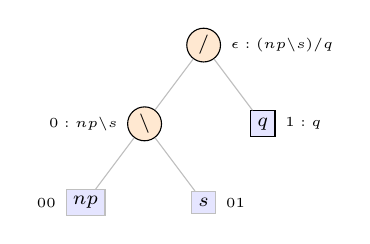
\begin{tikzpicture}[
  level distance=1.0cm,
  every node/.style={font=\scriptsize},
  cons/.style={circle,draw,fill=orange!18,inner sep=1.5pt},
  atom/.style={rectangle,draw,fill=blue!10,inner sep=2.5pt},
  edge from parent/.style={draw,gray!50},
]
\node[cons,label=right:{\tiny $\epsilon:(np\bs s)/q$}] {/}
  child {node[cons,label=left:{\tiny $0:np\bs s$}] {$\bs$}
    child {node[atom,label=left:{\tiny $00$}] {$np$}}
    child {node[atom,label=right:{\tiny $01$}] {$s$}}
  }
  child {node[atom,label=right:{\tiny $1:q$}] {$q$}};
\end{tikzpicture}
\end{center}

\smallskip
位置 $\epsilon$ と $0$ は constructor occurrence（$/$ と $\bs$），
位置 $1,00,01$ は原子（atom）である．
\end{verifybox}

\section{メタ変数コピー}

各規則スキームの $A,B,C$ をメタ変数と呼ぶ．
規則インスタンス $\rho$ におけるメタ変数 $X$ の各出現を\textbf{メタ変数コピー}と呼び，
代入された範疇を $\sigma_\rho(X)$ と書く．

\begin{verifybox}
\textbf{【例：$B{>}$ におけるメタ変数コピー】}
規則 $B{>}$（$C/B,\,B/A\Rightarrow C/A$）のインスタンスで
$\sigma(C)=s$，$\sigma(B)=np$，$\sigma(A)=n$ とすると
$s/np,\;np/n \Rightarrow s/n$．各メタ変数のコピーは：

\medskip
\begin{center}
\begin{tikzpicture}[
  every node/.style={font=\scriptsize},
  prem/.style={draw,rounded corners=2pt,minimum width=1.6cm,
               minimum height=0.6cm,fill=white},
]
\node[prem] (l) {$s/np$};
\node[prem,right=0.6cm of l] (r) {$np/n$};
\node[prem,below=1.0cm of $(l)!0.5!(r)$] (c) {$s/n$};
\draw[gray!50] (l.south) -- (c.north);
\draw[gray!50] (r.south) -- (c.north);
\node[right=1.2cm of r,align=left] {
  メタ変数 $C{=}s$：左前提と結論に各1コピー\\
  メタ変数 $B{=}np$：両前提に各1コピー\\
  メタ変数 $A{=}n$：右前提と結論に各1コピー
};
\end{tikzpicture}
\end{center}

\smallskip
ここでは $\sigma$ がすべて原子なので各コピーは内部 constructor を持たないが，
$\sigma(C)$ が複合範疇なら結論側の $C$ コピー内部にも constructor occurrence が現れる．
\end{verifybox}

%% ============================================================
\part{Trace graph}
%% ============================================================

\section{Trace edge}
\label{sec:trace}

\begin{definition}[trace edge]
導出図 $D$ の二 occurrence $(v,s)$，$(w,t)$ の間に \textbf{trace edge} を張るのは，
ある規則インスタンス $\rho$ と同じメタ変数 $X$ の二コピーがあり，
$(v,s)$ と $(w,t)$ がそれぞれその二コピー内部の\textbf{同じ相対位置}にある場合である．
このとき $(v,s)\sim_\rho(w,t)$ と書く．
\end{definition}

\textbf{Trace graph} は頂点集合 $\Occ(D)$，辺集合をすべての trace edge とする無向グラフである．

\medskip
\noindent\textbf{設計判断．}
型上げ $A\Rightarrow C/(A\bs C)$ が\textbf{新しく導入した}外側 $/$ と内側 $\bs$ 自体は，
どのメタ変数コピーの内部 occurrence でもないので，それらの間には trace edge を張らない．
前提の $A$ と結論中の $A$（内側）は同じメタ変数なのでその内部 occurrence は結ばれる．
結論中の二つの $C$ も同様．

\begin{verifybox}
\textbf{【検証：例3 の導出木と trace graph】}

導出：$n_1=a$（葉）$\xRightarrow{T{>}}$ $n_2=s/(a\bs s)$ $\xRightarrow{T{>}}$ $n_3=s/((s/(a\bs s))\bs s)$（深さ4），$n_3,n_4\xRightarrow{>}n_5=s$（根），$n_4=(s/(a\bs s))\bs s$（葉）．

\medskip
\begin{center}
\begin{prooftree}
  \hypo{a}
  \infer1[$(T{>},\,C{=}s)$]{s/(a\bs s)}
  \infer1[$(T{>},\,C{=}s)$]{s/\bigl((s/(a\bs s))\bs s\bigr)}
  \hypo{(s/(a\bs s))\bs s}
  \infer2[$(>)$]{s}
\end{prooftree}
\end{center}

\medskip
下図に trace graph を示す．
\textbf{青丸}が visible occurrence，\textbf{橙丸}が invisible occurrence，
破線囲みが invisible trace piece（$P_1, P_2, P_3$）．
矢印は trace edge（双方向）．

\medskip
\begin{center}
\begin{tikzpicture}[
  node distance=0.85cm and 2.0cm,
  every node/.style={font=\scriptsize},
]
%% ---- Column: n2 (invisible) ----
\node[inv] (n2e)  {$n_2,\epsilon$};
\node[inv,below=of n2e] (n2o)  {$n_2,1$};

%% ---- Column: n3 (mix) ----
\node[vis, right=2.8cm of n2e] (n3e)  {$n_3,\epsilon$};
\node[inv, below=of n3e] (n3o)  {$n_3,1$};
\node[inv, below=of n3o] (n3t)  {$n_3,10$};
\node[inv, below=of n3t] (n3h)  {$n_3,101$};

%% ---- Column: n4 (leaf = all visible) ----
\node[vis, right=2.8cm of n3e] (n4e)  {$n_4,\epsilon$};
\node[vis, below=of n4e]        (n4z)  {$n_4,0$};
\node[vis, below=of n4z]        (n4zo) {$n_4,01$};

%% ---- n5 root ----
\node[vis, right=1.4cm of n4e]  (n5e)  {$n_5,\epsilon$};

%% ---- trace edges ----
\draw[traceedgebi] (n2e) -- node[above,font=\tiny]{外側$T_>$の$A$} (n3t);
\draw[traceedgebi] (n2o) -- node[below,font=\tiny]{内側$T_>$の$A$} (n3h);
\draw[traceedgebi] (n3o) -- (n4e);
\draw[traceedgebi] (n3t) -- (n4z);
\draw[traceedgebi] (n3h) -- (n4zo);

%% ---- invisible piece highlights ----
\begin{scope}[on background layer]
  \node[pieceA,fit=(n2e)(n3t),inner sep=5pt,
        label={[font=\tiny,teal!70!black]above:$P_2$}] {};
  \node[pieceB,fit=(n2o)(n3h),inner sep=5pt,
        label={[font=\tiny,red!70!black]below:$P_1$}] {};
  \node[pieceC,fit=(n3o),inner sep=5pt,
        label={[font=\tiny,violet!70!black]right:$P_3$}] {};
\end{scope}

%% ---- node labels (derivation position) ----
\node[above=0.15cm of n2e,font=\tiny,gray]  {節点$n_2$};
\node[above=0.15cm of n3e,font=\tiny,gray]  {節点$n_3$};
\node[above=0.15cm of n4e,font=\tiny,gray]  {節点$n_4$（葉）};
\node[above=0.15cm of n5e,font=\tiny,gray]  {$n_5$（根）};

%% ---- legend ----
\node[vis,below=1.5cm of n3h] (lv) {};
\node[right=3pt of lv] {visible};
\node[inv,right=1.5cm of lv] (li) {};
\node[right=3pt of li] {invisible};
\draw[traceedgebi,right=3cm of lv] ($(lv)+(3.2cm,0)$) -- ++(1.0cm,0)
  node[right]{trace edge};
\end{tikzpicture}
\end{center}

\smallskip
Trace edge の一覧（計算機検証済み）：
$(n_2,\epsilon)\sim(n_3,10)$，$(n_2,1)\sim(n_3,101)$，
$(n_3,1)\sim(n_4,\epsilon)$，$(n_3,10)\sim(n_4,0)$，$(n_3,101)\sim(n_4,01)$．
型上げの骨格 $(n_3,\epsilon)$，$(n_3,1)$ は trace edge を持たない（メタ変数内部でない）．
\end{verifybox}

\section{Visible occurrence}
\label{sec:visible}

\begin{definition}[visible / invisible]
導出 occurrence $(v,s)$ が \textbf{visible} であるとは次のいずれかが成り立つこと：
\begin{enumerate}
  \item $v$ が葉である．
  \item $v$ が根である．
  \item $(v,s)$ が二項規則の \textbf{principal constructor} である（二項規則が直接見る最外スラッシュ）．
\end{enumerate}
Application $C/B,B\Rightarrow C$ では左前提の根 $/$；
$A,A\bs C\Rightarrow C$ では右前提の根 $\bs$；
Composition $C/B,B/A\Rightarrow C/A$ では左・右前提・結論の根 $/$，計3個．
型上げが導入した constructor は，それだけでは visible ではない．
visible でない occurrence を \textbf{invisible} と呼ぶ．
\end{definition}

\section{Visible occurrence の個数上界 $V$}
\label{sec:V}

入力の constructor 総数 $\sum_{i=1}^{n}c(x_i)$，目標は $c(y)$，
二項規則はちょうど $n-1$ 回・各回の principal は高々3個なので，
\[
  V = \sum_{i=1}^{n}c(x_i) + c(y) + 3(n-1).
\]

\begin{verifybox}
\textbf{【検証：$V$ の計算】}
例3（入力 $a$ と $(s/(a\bs s))\bs s$，目標 $s$，$n=2$）では
$\sum_i c(x_i)=0+3=3$，$c(y)=0$，$3(n-1)=3$，$V=6$（計算機確認済み）．
\end{verifybox}

\section{Invisible trace piece}
\label{sec:piece}

trace graph から visible occurrence をすべて取り除き，
残ったグラフの連結成分を \textbf{invisible trace piece} と呼ぶ．

\begin{verifybox}
\textbf{【検証：例3 の invisible piece】}
例3 の trace graph（前図）から visible occurrence（青丸）を除いた残りの連結成分は
$P_1=\{(n_2,1),(n_3,101)\}$，$P_2=\{(n_2,\epsilon),(n_3,10)\}$，$P_3=\{(n_3,1)\}$ の3つ．
各 piece は節点 $n_3$ の branch を高々1回しか横切らない（計算機確認済み）．
\end{verifybox}

%% ============================================================
\part{Interface state と trace degree}
%% ============================================================

\section{Interface state}
\label{sec:iface}

\begin{definition}[interface state]
固定した中間範疇 $A_v$ と root-to-leaf branch $\beta$ について，
branch 上の \textbf{invisible} occurrence $o=(v,s)$ の
\textbf{interface state} を
$\st_\beta(o) = (\ell,\,\delta,\,\pi^-,\,\pi^+)$
と定める．
$\ell\in\{/,\bs\}$ は occurrence のラベル，
$\delta\in\{0,1\}$ は branch がその constructor の左子・右子のどちらへ進むか，
$\pi^-$ は $A_v$ を生成した下側規則でのポート型，
$\pi^+$ は消費する上側規則でのポート型である．
\end{definition}

葉と根は visible なので invisible occurrence には必ず上下の規則が存在し，$\pi^-,\pi^+$ が定義される．
interface state の全体は有限集合であり，その個数を $q$ と書く．

\begin{verifybox}
\textbf{【検証：interface state は branch 上で変化する】}
$Z=s/((s/(a\bs s))\bs s)$（節点 $n_3$）の葉 $a$ への branch 上の constructors の
$(\ell,\delta)$ を計算機で列挙すると変化する：

\medskip
\begin{center}
\begin{tikzpicture}[
  node distance=0.5cm,
  bnode/.style={draw,rounded corners=2pt,minimum width=1.8cm,
                minimum height=0.55cm,font=\scriptsize,fill=white},
  every node/.style={font=\scriptsize},
]
\node[bnode,fill=orange!18,draw=orange!65] (e)   {$\epsilon\;:\;(/,1)$};
\node[bnode,fill=orange!18,draw=orange!65,below=of e] (o)  {$1\;:\;(\bs,0)$};
\node[bnode,fill=orange!18,draw=orange!65,below=of o] (t)  {$10\;:\;(/,1)$};
\node[bnode,fill=orange!18,draw=orange!65,below=of t] (h)  {$101\;:\;(\bs,0)$};
\node[draw=none,below=0.3cm of h,text=gray] {$\vdots$（葉 $a$）};
\draw[-{Stealth[length=4pt]},gray!60] (e) -- (o)
  node[midway,right=3pt]{branch 進行方向};
\draw[-{Stealth[length=4pt]},gray!60] (o) -- (t);
\draw[-{Stealth[length=4pt]},gray!60] (t) -- (h);

\node[right=3.5cm of e,align=left,font=\scriptsize] (ex) {
  $(\ell,\delta)$ の値は\\branch に沿って変化する．\\
  piece と interface state の両方が\\
  一致して初めて repeatable pair\\
  になる（\S\ref{sec:depth}参照）．
};
\end{tikzpicture}
\end{center}
\end{verifybox}

\section{Trace degree 定数 $r$}

各 occurrence の trace degree（trace graph における次数）は
規則集合 $\R$ のみから決まる有限定数 $r$ で上から抑えられる．

%% ============================================================
\part{Band contraction}
%% ============================================================

\section{One-hole context と branch context}

\textbf{one-hole context} $E[\cdot]$ とは範疇の1箇所を穴に置き換えたもの．
位置 $s\prec t$ のとき $A|_s=L_{s,t}[A|_t]$ と書け，この $L_{s,t}[\cdot]$ を \textbf{branch context} と呼ぶ．

\section{Transport-closed band}
\label{sec:band}

\begin{definition}[transport-closed band]
導出図 $D$ の \textbf{transport-closed band} とは，
いくつかの節点 $v$ について位置対 $s_v\prec t_v$ を指定した有限集合で，
$A_v = E_v[L_v[Z_v]]$（$Z_v=A_v|_{t_v}$）と書け，次を満たすもの：
\begin{enumerate}
  \item 各 $L_v[\cdot]$ は少なくとも1個の constructor を含む．
  \item 各 $L_v[\cdot]$ に含まれる constructor occurrence はすべて invisible．
  \item ある規則インスタンスでメタ変数 $X$ の一コピー内部で $L[\cdot]$ が削除対象なら，
        同じインスタンスの $X$ の\textbf{すべてのコピー}内部でも同じ相対位置の $L[\cdot]$ が削除対象．
  \item 別のメタ変数 $Y\neq X$ のコピーには影響しない．
  \item 葉と根の範疇には削除対象がない．
\end{enumerate}
\end{definition}

\section{Band contraction の操作}

band $B$ について，各指定節点で $A_v=E_v[L_v[Z_v]]$ を $A'_v=E_v[Z_v]$ に置き換えたものを $D/B$ と書く．

\section{Transport-closed band は縮約できる}

\begin{lemma}
\label{lem:band-correct}
$B$ が $D$ の transport-closed band なら，
$D/B$ は同じ入力列と同じ目標範疇を持つ正しい導出図であり，$\mu(D/B)<\mu(D)$．
\end{lemma}

\begin{proof}
各規則インスタンスが縮約後も同じ規則スキームのインスタンスであることを示す．

$B{>}$（$C/B,\,B/A\Rightarrow C/A$）で $C$ 内部に削除対象がある場合：
\[
  E[L[Z]]/B,\;B/A \Rightarrow E[L[Z]]/A
  \;\longrightarrow\;
  E[Z]/B,\;B/A \Rightarrow E[Z]/A.
\]
再び $B{>}$．$B,A$ 内部の削除も同様．Application，composition，crossed composition も
各メタ変数コピーに一様縮約するだけなので規則を保つ．
$Bx{>}$（$C/B,\,A\bs B\Rightarrow A\bs C$）で $B$ 内部を縮約する例：
\[
  C/E[L[Z]],\;A\bs E[L[Z]] \Rightarrow A\bs C
  \;\longrightarrow\;
  C/E[Z],\;A\bs E[Z] \Rightarrow A\bs C.
\]
$T{>}$（$A\Rightarrow C/(A\bs C)$）で $A$ 内部を縮約：
\[
  E[L[Z]] \Rightarrow C/(E[L[Z]]\bs C)
  \;\longrightarrow\;
  E[Z] \Rightarrow C/(E[Z]\bs C).
\]
条件5より葉と根は不変なので入力列と目標は同じ．
各 $L_v[\cdot]$ は少なくとも1個の constructor を含むので $\mu(D/B)<\mu(D)$．
\end{proof}

\section{Repeatable pair から band ができる}

\begin{definition}[repeatable pair]
$D$，節点 $v$，branch $\beta$ 上の二 invisible occurrence $o=(v,s)$，$o'=(v,t)$（$s\prec t$）が
\begin{enumerate}
  \item 同じ invisible trace piece $P$ に属する，
  \item $\st_\beta(o)=\st_\beta(o')$，
  \item $s$ と $t$ の間の branch segment に visible occurrence がない，
\end{enumerate}
を満たすとき，$(o,o')$ を \textbf{repeatable pair} と呼ぶ．
\end{definition}

\begin{lemma}
\label{lem:rep-band}
$D$ に repeatable pair が存在するなら，$D$ には transport-closed band が存在する．
\end{lemma}

\begin{proof}
$A_v|_s=L[A_v|_t]$ と書く．$o,o'$ は同じ piece に属するので trace graph に $o$ から $o'$ への path がある．
trace edge は同じメタ変数コピー間の同じ相対位置を結ぶので，$L[\cdot]$ は trace path に沿って
同じメタ変数コピーの他 occurrence へ一意に transport される．
interface state が等しいため transport は各規則インスタンスで閉じる．
$o,o'$ は invisible・$s,t$ 間に visible なし・$s\prec t$ ゆえ $L[\cdot]$ は少なくとも1個の constructor を含む．
葉と根は visible なので band は葉・根に触れない．
よって transport された branch contexts の族が transport-closed band を成す．
\end{proof}

\begin{verifybox}
\textbf{【検証：band contraction の before/after】}

型上げ2段の冗長導出（long）と縮約後の短い導出（short）を対比する（計算機で valid 確認済み）．

\medskip
\begin{center}
\begin{tabular}{cc}
\textbf{Long（$\mu=9$）} & \textbf{Short（$\mu=5$）} \\[4pt]
\begin{prooftree}
  \hypo{a}
  \infer1[$(T{>},\,C{=}c)$]{c/(a\bs c)}
  \infer1[$(T{>},\,C{=}c)$]{c/\bigl((c/(a\bs c))\bs c\bigr)}
  \hypo{(c/(a\bs c))\bs c}
  \infer2[$(>)$]{c}
\end{prooftree}
&
\begin{prooftree}
  \hypo{a}
  \infer1[$(T{>},\,C{=}c)$]{c/(a\bs c)}
  \hypo{(c/(a\bs c))\bs c}
  \infer2[$(<)$]{c}
\end{prooftree}
\end{tabular}
\end{center}

\medskip
Long の中間範疇 $Y=c/\bigl((c/(a\bs c))\bs c\bigr)$ は，
$Y = c/\bigl(\underbrace{(c/(a\bs c))}_{X}\bs c\bigr)$ と分解できる．
削除層 $L[\cdot]=c/([\cdot]\bs c)$ を取り除くと $X=c/(a\bs c)$（Short の中間範疇）になる．

\medskip
下図に「deep $Y$ の branch（根 $\to$ 葉 $a$）上で，どの位置が外側骨格 $E[\cdot]$・
削除層 $L[\cdot]$・残す中身 $Z$ に対応するか」を可視化する．
分解は $E[\cdot]=c/([\cdot]\bs c)$（穴は位置 $10$），$L[\cdot]=c/([\cdot]\bs c)$，$Z=a$ で，
$E[L[Z]]=Y$，$E[Z]=X$ が成り立つ（計算機確認済み）．

\medskip
\begin{center}
\begin{tikzpicture}[
  every node/.style={font=\scriptsize},
  ptbox/.style={circle,draw,minimum size=0.5cm,inner sep=0pt,fill=white},
  Epos/.style={ptbox,fill=blue!15,draw=blue!55,thick},
  Lpos/.style={ptbox,fill=red!14,draw=red!60},
  Zpos/.style={ptbox,fill=orange!20,draw=orange!65},
  lbl/.style={font=\scriptsize,anchor=west},
]
%% ===== 縮約前 Y：branch を縦に。位置 ε,1,10,101,1010 =====
\def\yA{0} \def\yB{-1.0} \def\yC{-2.0} \def\yD{-3.0} \def\yE{-4.0}
\draw[gray!40,line width=1.3pt] (0,\yA) -- (0,\yE);

\node[Epos] (pe)  at (0,\yA) {};
\node[Epos] (p1)  at (0,\yB) {};
\node[Lpos] (p10) at (0,\yC) {};
\node[Lpos] (p101)at (0,\yD) {};
\node[Zpos] (pz)  at (0,\yE) {};

\node[lbl] at (0.45,\yA) {位置 $\epsilon:\,/$\;\; visible（$E$ 外側）};
\node[lbl] at (0.45,\yB) {位置 $1:\,\bs$\;\; invisible（$E$ 内側）};
\node[lbl] at (0.45,\yC) {位置 $10:\,/$\;\; invisible（$L$ 外側）};
\node[lbl] at (0.45,\yD) {位置 $101:\,\bs$\;\; invisible（$L$ 内側）};
\node[lbl] at (0.45,\yE) {位置 $1010:\,a$\;\; （$Z$，葉へ）};

%% E の brace（位置 ε,1 を囲む：左側）
\draw[decorate,decoration={brace,amplitude=4pt},blue!55,thick]
  (-0.45,\yB-0.32) -- (-0.45,\yA+0.32)
  node[midway,left=5pt,blue!60!black,align=center]{骨格\\$E[\cdot]$};
%% L の brace（位置 10,101 を囲む：左側）
\draw[decorate,decoration={brace,amplitude=4pt},red!60,thick]
  (-0.45,\yD-0.32) -- (-0.45,\yC+0.32)
  node[midway,left=5pt,red!70!black,align=center]{削除層\\$L[\cdot]$};

\node[above=0.15cm of pe,font=\scriptsize,gray]{縮約前 $Y$（深さ4）};

%% ===== contraction arrow =====
\draw[-{Stealth[length=6pt,width=5pt]},thick,red!55]
  (3.6,\yC) -- node[above,font=\scriptsize,align=center]{band\\contraction\\（$L$を削除）} ++(1.8,0);

%% ===== 縮約後 X：位置 ε,1,10 =====
\begin{scope}[shift={(7.0,0)}]
\def\wA{0} \def\wB{-1.0} \def\wC{-2.0}
\draw[gray!40,line width=1.3pt] (0,\wA) -- (0,\wC);
\node[Epos] (qe) at (0,\wA) {};
\node[Epos] (q1) at (0,\wB) {};
\node[Zpos] (qz) at (0,\wC) {};
\node[lbl] at (0.45,\wA) {位置 $\epsilon:\,/$};
\node[lbl] at (0.45,\wB) {位置 $1:\,\bs$};
\node[lbl] at (0.45,\wC) {位置 $10:\,a$（葉へ）};
\node[above=0.15cm of qe,font=\scriptsize,gray]{縮約後 $X$（深さ2）};
\end{scope}
\end{tikzpicture}
\end{center}

\smallskip
削除層 $L[\cdot]$ は位置 $10$（外側 $/$）と $101$（内側 $\bs$）を占める invisible occurrence であり，
これを取り除くと骨格 $E[\cdot]$ の穴に $Z=a$ がはまって $X=c/(a\bs c)$ になる．
位置 $1$ の $\bs$ も位置 $10,101$ も，この導出（long）では葉でも根でも principal でもないため invisible である
（$Y$ は $>$ の左前提で，principal は位置 $\epsilon$ の $/$ のみ）．
\end{verifybox}

\begin{lemma}[Band-contraction lemma]
\label{lem:band-contract}
$D$ に repeatable pair が存在するなら，
同じ入力列と同じ目標範疇を持つ導出図 $D'$ が存在し $\mu(D')<\mu(D)$．
\end{lemma}

\begin{proof}
補題~\ref{lem:rep-band} より transport-closed band $B$ が得られ，
補題~\ref{lem:band-correct} より $D'=D/B$ が所望の導出である．
\end{proof}

%% ============================================================
\part{最小導出}
%% ============================================================

\section{$\mu$-最小成功導出}
\label{sec:minimal}

成功導出が存在すると仮定する．
補題~\ref{lem:atom} より途中の原子がすべて $\Sig$ に属する成功導出だけを考えればよい．
その中で $\mu(D)$ が最小のものを $\Dmin$ と書く．

\begin{corollary}
\label{cor:minimal}
$\Dmin$ には repeatable pair が存在しない．
\end{corollary}

\begin{proof}
もし存在すれば，補題~\ref{lem:band-contract} により $\mu(D')<\mu(\Dmin)$ となる成功導出 $D'$ が存在し，最小性に反する．
\end{proof}

\begin{verifybox}
\textbf{【検証：$\mu$ の比較】}
Long と Short の $\mu$ を計算機で確認：
$\mu(\text{long})=9$，$\mu(\text{short})=5$，$\mu(\text{short})<\mu(\text{long})$．
long は $\mu$-最小でないので，long で band が閉じないことは証明と矛盾しない．
\end{verifybox}

\section{Boundary-free piece は最小導出に存在しない}

\begin{definition}[visible boundary]
invisible trace piece $P$ が \textbf{visible boundary} を持つとは，
ある visible occurrence $u$ と $P$ 内の occurrence $o$ の間に trace edge があることをいう．
\end{definition}

\begin{lemma}
\label{lem:no-boundary-free}
$\Dmin$ において，visible boundary を持たない invisible trace piece は存在しない．
\end{lemma}

\begin{proof}
visible boundary を持たない invisible trace piece $P$ があると仮定する．
$P$ の occurrence は導出の外部（入力・目標・principal 使用）から観測されない．
$P$ の occurrence を含む最小の部分範疇を各メタ変数コピーで一様に固定原子 $p_\ast\in\Sig$ に置き換えると，
補題~\ref{lem:band-correct} と同じ一様置換の議論により全規則が保存される．
少なくとも1個の constructor occurrence が原子に置き換わるので $\mu$ が真に減少し，最小性に反する．
\end{proof}

\section{Invisible trace piece の個数上界}

visible occurrence の総数は高々 $V$，trace degree は高々 $r$．
補題~\ref{lem:no-boundary-free} より $\Dmin$ の全 invisible piece が visible boundary を持つので，
$\Dmin$ の invisible piece 総数は高々 $rV$．

%% ============================================================
\part{深さ上界}
%% ============================================================

\section{深さ上界の数え上げ}
\label{sec:depth}

任意の中間範疇 $A_v$ と root-to-leaf branch $\beta$ を固定する．
branch 上の任意の二点は prefix で全順序に並ぶので，同じ branch 上の二 occurrence は必ず祖先関係にある．

\medskip
\noindent\textbf{Visible．}
branch 上に高々 $V$ 個．
これらで branch は高々 $V+1$ 個の \textbf{visible-free zone} に分割される．

\medskip
\noindent\textbf{Invisible（一 zone あたり）．}
一 zone 内で，同じ invisible piece に属し同じ interface state を持つ occurrence が二つあれば
repeatable pair になるが，$\Dmin$ にはない（系~\ref{cor:minimal}）．
一 zone 内での各 (piece, interface state) の組は高々一回，組は高々 $rV\times q$ なので，
一 zone 内の invisible occurrence は高々 $q\cdot rV$．

\medskip
\noindent\textbf{合計．}
\[
  d(A_v) \le V + qrV(V+1) =: H(\Gamma,y).
\]
$q,r$ は $\R$ のみから決まる有限定数，$V$ は入力と目標から計算できる．

\begin{verifybox}
\textbf{【可視化：branch 上の visible/invisible/zone 分割】}

下図は branch（縦の脊柱，模式図）を表す．\textbf{青丸}の visible occurrence $v_1,\dots,v_5$ が
branch を区切り，その間の各区間が \textbf{visible-free zone}（黄帯）である．
zone 内の \textbf{橙丸}が invisible occurrence．visible が $V$ 個なら zone は高々 $V+1$ 個．

\medskip
\begin{center}
\begin{tikzpicture}[
  every node/.style={font=\scriptsize},
  occ/.style={circle,minimum size=0.32cm,draw,inner sep=0pt},
]
%% visible occurrence の y 座標（等間隔）
\def\sep{1.9}
\def\vA{0}
\pgfmathsetmacro\vB{-\sep}
\pgfmathsetmacro\vC{-2*\sep}
\pgfmathsetmacro\vD{-3*\sep}
\pgfmathsetmacro\vE{-4*\sep}

% spine
\draw[gray!40,line width=1.4pt] (0,\vA) -- (0,\vE);

%% zone 帯：隣接する visible の「内側」を塗る（丸の半径ぶん控える）
\def\pad{0.28}
\foreach \top/\bot/\num in {\vA/\vB/1, \vB/\vC/2, \vC/\vD/3, \vD/\vE/4}{
  \fill[yellow!22] (-0.45,{\top-\pad}) rectangle (0.45,{\bot+\pad});
  \node[right=0.62cm,font=\tiny,gray] at (0,{(\top+\bot)/2}) {zone \num};
}

%% invisible occurrences：各 zone の中央付近に3個ずつ、帯の範囲内に収める
\foreach \top/\bot in {\vA/\vB, \vB/\vC, \vC/\vD, \vD/\vE}{
  \pgfmathsetmacro\mid{(\top+\bot)/2}
  \node[occ,inv] at (0,{\mid+0.45}) {};
  \node[occ,inv] at (0,{\mid}) {};
  \node[occ,inv] at (0,{\mid-0.45}) {};
}

%% visible occurrences（境界。invisible より前面）
\foreach \y/\lbl in {\vA/{$v_1$}, \vB/{$v_2$}, \vC/{$v_3$}, \vD/{$v_4$}, \vE/{$v_5$}}{
  \node[occ,vis] at (0,\y) {};
  \node[left=5pt,blue!60!black] at (0,\y) {\lbl};
}

%% zone 2 への brace（高々 qrV 個）
\draw[decorate,decoration={brace,mirror,amplitude=4pt},teal!65,thick]
  (0.55,{\vC+\pad}) -- (0.55,{\vB-\pad})
  node[midway,right=6pt,teal!70!black,align=left]{各 zone に\\高々 $qrV$ 個};

%% legend（右下、脊柱と十分離す）
\begin{scope}[shift={(4.2,\vD)}]
  \node[occ,vis] (lv) at (0,0) {};
  \node[right=4pt] at (0,0) {visible（zone 境界）};
  \node[occ,inv] (li) at (0,-0.55) {};
  \node[right=4pt] at (0,-0.55) {invisible};
  \fill[yellow!30,draw=yellow!60] (-0.16,-1.26) rectangle (0.16,-0.94);
  \node[right=4pt] at (0,-1.1) {zone};
\end{scope}
\end{tikzpicture}
\end{center}

\smallskip
\textbf{なぜ積 $q\cdot rV$ か．}
例3 の $Z$ の branch 上で $(\ell,\delta)=(/,1)$ の occurrence が $\epsilon$ と $10$ の2つあるが，
$(n_3,\epsilon)$ は visible（$>$ の principal）で piece に属さず（孤立），$(n_3,10)\in P_2$．
$(\ell,\delta)$ が一致しても piece が違えば repeatable pair にならない——piece（高々 $rV$ 種）と
interface state（高々 $q$ 種）の\textbf{両方}が一致して初めて削れる．
これが一 zone 内の invisible 上界が積 $q\cdot rV$ になる理由である（計算機確認済み）．
\end{verifybox}

%% ============================================================
\part{有界正規形と決定可能性}
\label{sec:chart}
%% ============================================================

\section{有界正規形定理}

\begin{theorem}[Bounded-category normal form]
\label{thm:bounded}
$x_1,\ldots,x_n\Rightarrow_{\R}^{*}y$ ならば，
途中の全範疇 $A$ について $\At(A)\subseteq\Sig$ かつ $d(A)\le H(\Gamma,y)$ を満たす
同じ入力列・目標の導出 $D'$ が存在する．
\end{theorem}

\begin{proof}
補題~\ref{lem:atom} より $\At(A)\subseteq\Sig$ の成功導出があり，その $\mu$-最小のものを $\Dmin$ とする．
系~\ref{cor:minimal} より repeatable pair なし，
補題~\ref{lem:no-boundary-free} より boundary-free invisible piece なし．
\S\ref{sec:depth} の数え上げにより $d(A)\le H(\Gamma,y)$．$D'=\Dmin$．
\end{proof}

\section{有限候補範疇集合}

\[
  K_{\Gamma,y} = \{\,A\mid \At(A)\subseteq\Sig,\;d(A)\le H(\Gamma,y)\,\}.
\]
$\Sig$ が有限・深さ有界なので $K_{\Gamma,y}$ は有限かつ機械的に列挙可能．

\section{有限 chart algorithm}
\label{sec:chart-alg}

各区間 $[i,j)$ に有限集合 $\Chart[i,j]\subseteq K_{\Gamma,y}$ を持つ chart を作り，
以下の closure を固定点まで繰り返す．

\medskip
\noindent\textbf{Unary closure．}
$A\in\Chart[i,j]$ かつ $C/(A\bs C)\in K_{\Gamma,y}$ なら追加；$(C/A)\bs C\in K_{\Gamma,y}$ なら同様．

\medskip
\noindent\textbf{Binary closure．}
$A\in\Chart[i,k]$，$B\in\Chart[k,j]$，六つの二項規則のいずれかで $C\in K_{\Gamma,y}$ が得られれば追加．

\begin{verifybox}
\textbf{【例：例1 の chart trace】}
入力 $a,\;(a\bs s)/b,\;b$（$n=3$），目標 $s$ に対する chart の充填過程
（計算機で再現済み）．区間 $[i,j)$ は語 $x_{i+1},\dots,x_j$ を覆う．

\medskip
\begin{center}
\begin{tikzpicture}[
  every node/.style={font=\scriptsize},
  cell/.style={draw,minimum width=2.3cm,minimum height=0.7cm,
               rounded corners=2pt,fill=white,align=center},
  filled/.style={cell,fill=green!10,draw=green!55},
  goalcell/.style={cell,fill=blue!12,draw=blue!60,thick},
]
% bottom row: leaves
\node[filled] (c01) at (0,0)   {$[0,1)$\\ $a,\;s/(a\bs s)$};
\node[filled] (c12) at (2.6,0) {$[1,2)$\\ $(a\bs s)/b$};
\node[filled] (c23) at (5.2,0) {$[2,3)$\\ $b$};
% middle row
\node[filled] (c02) at (1.3,1.2) {$[0,2)$\\ $s/b$};
% top
\node[goalcell] (c03) at (2.6,2.4) {$[0,3)$\\ $\boxed{s}$};

% arrows showing closure
\draw[-{Stealth[length=4pt]},teal!60] (c01) -- node[left=1pt,font=\tiny]{$B{>}$} (c02);
\draw[-{Stealth[length=4pt]},teal!60] (c12) -- (c02);
\draw[-{Stealth[length=4pt]},blue!60] (c02) -- node[left=1pt,font=\tiny]{$>$} (c03);
\draw[-{Stealth[length=4pt]},blue!60] (c23) to[bend right=15] (c03);

\node[right=0.3cm of c03,align=left,font=\tiny,gray]{
  $\Chart[0,1]$ で unary closure が\\
  $T{>}(a){=}s/(a\bs s)$ を追加，\\
  $B{>}$ で $\Chart[0,2]{=}s/b$，\\
  $>$ で $\Chart[0,3]\ni s$．
};
\end{tikzpicture}
\end{center}

\smallskip
$s\in\Chart[0,3]$ となり，導出可能性が chart 上で確認される．
\end{verifybox}

\section{停止性・健全性・完全性}

chart item 総数は有限なので closure は必ず停止する（停止性）．
item 追加順の帰納法により，chart に入る item は実際に導出可能（健全性）．
定理~\ref{thm:bounded} より途中の全範疇が $K_{\Gamma,y}$ に属する成功導出 $D'$ が存在し，
$D'$ への構造帰納法により $y\in\Chart[0,n]$（完全性）．

\section{決定可能性}

健全性と完全性より，
\[
  x_1,\ldots,x_n\Rightarrow_{\R}^{*}y
  \quad\Longleftrightarrow\quad
  y\in\Chart[0,n].
\]
右辺は有限集合上の固定点計算で判定でき，停止する．

\bigskip
\begin{tcolorbox}[
  enhanced, colback=white, colframe=black,
  boxrule=1pt, arc=2pt,
  left=8pt, right=8pt, top=6pt, bottom=6pt,
]
\[
  x_1,\ldots,x_n
  \Rightarrow_{\{<,>,T{<},T{>},B{<},B{>},Bx{<},Bx{>}\}}^{*}
  y
  \quad\text{は判定可能である．}
\]
\end{tcolorbox}
\qed

%% ============================================================
\section*{証明の要点}
\addcontentsline{toc}{section}{証明の要点}
%% ============================================================

第一に，入力と目標に現れない原子は準同型で潰せる（補題~\ref{lem:atom}）．

第二に，$\mu$-最小成功導出では外から見えない trace の反復は band contraction で削れる
（補題~\ref{lem:band-correct}--\ref{lem:band-contract}，系~\ref{cor:minimal}）．
型上げの骨格を trace edge から外す設計（\S\ref{sec:trace}）が，
「型上げを重ねただけの見かけの深さ」を repeatable pair として誤検出しないことを保証する．

第三に，可視化した zone 分割（\S\ref{sec:depth}）の通り，
visible occurrence が $V$ 個・invisible piece が $rV$ 個・interface state が $q$ 種の積として，
中間範疇の深さは $H(\Gamma,y)=V+qrV(V+1)$ で有界になる．

%% ============================================================
\appendix
\section{検証に用いた具体例の要約}
%% ============================================================

\begin{center}
\renewcommand{\arraystretch}{1.4}
\begin{tabular}{lll}
\toprule
例 & 導出 & 確認内容 \\
\midrule
例1 & $a,\;(a\bs s)/b,\;b\Rightarrow s$ & 型上げ＋合成の valid 成功導出 \\
例2 long & $a\Rightarrow X\Rightarrow Y$;\;$Y,w_2\Rightarrow c$ & $\mu=9$，band が葉に当たる \\
例2 short & $a\Rightarrow X$;\;$X,w_2\Rightarrow c$ & $\mu=5<9$，同入力の短い導出 \\
例3 & $a\Rightarrow A\Rightarrow Z$;\;$Z,n_4\Rightarrow s$ & 深さ4，$V=6$，invisible piece 3つ \\
\bottomrule
\end{tabular}
\end{center}

$X=c/(a\bs c)$，$Y=c/\bigl((c/(a\bs c))\bs c\bigr)$，$w_2=(c/(a\bs c))\bs c$，
$A=s/(a\bs s)$，$Z=s/\bigl((s/(a\bs s))\bs s\bigr)$，$n_4=(s/(a\bs s))\bs s$．

\end{document}
